% Asset ID: AS1GraphsTransformationsTikZ-004
% Source: CCEA AS1-AF-LO014, AS1-AF-LO015 + DrFrost points of intersection evidence
% Purpose: Show graph intersections and link them to solving f(x)=g(x)
\documentclass[tikz,border=8pt]{standalone}
\usepackage{pgfplots}
\pgfplotsset{compat=1.18}
\begin{document}
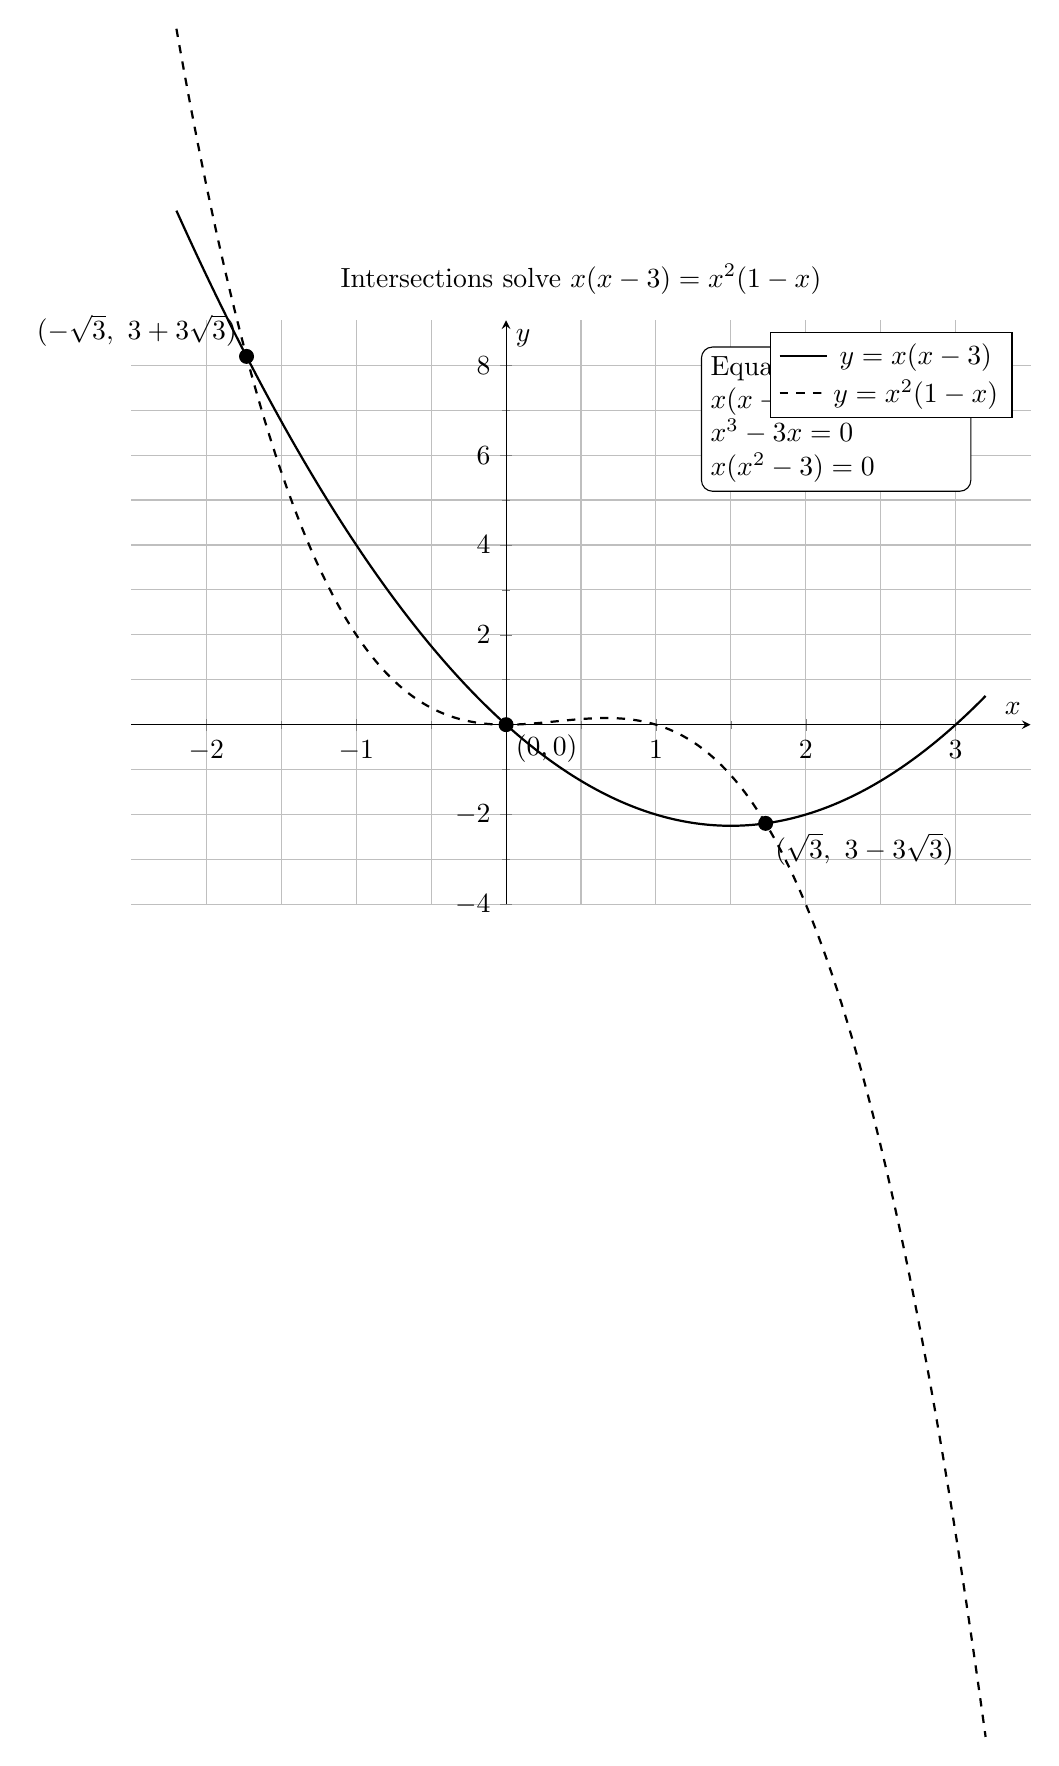
\begin{tikzpicture}
\begin{axis}[axis lines=middle,xmin=-2.5,xmax=3.5,ymin=-4,ymax=9,xlabel={$x$},ylabel={$y$},xtick={-2,-1,0,1,2,3},ytick={-4,-2,0,2,4,6,8},grid=both,minor tick num=1,width=13cm,height=9cm,samples=250,domain=-2.2:3.2,enlargelimits=false,clip=false,legend style={at={(0.98,0.98)},anchor=north east},title={Intersections solve $x(x-3)=x^2(1-x)$}]
\addplot[thick,smooth]{x*(x-3)};\addlegendentry{$y=x(x-3)$}
\addplot[thick,smooth,dashed]{x^2*(1-x)};\addlegendentry{$y=x^2(1-x)$}
\addplot[only marks,mark=*,mark size=2.5pt] coordinates{(0,0)};
\addplot[only marks,mark=*,mark size=2.5pt] coordinates{(-1.7320508076,8.196152423)(1.7320508076,-2.196152423)};
\node[anchor=south east] at (axis cs:-1.7320508076,8.196152423){$(-\sqrt3,\ 3+3\sqrt3)$};
\node[anchor=north west] at (axis cs:0,0){$(0,0)$};
\node[anchor=north west] at (axis cs:1.7320508076,-2.196152423){$(\sqrt3,\ 3-3\sqrt3)$};
\node[draw,rounded corners,fill=white,align=left,anchor=west] at (axis cs:1.3,6.8){Equate the graphs:\\$x(x-3)=x^2(1-x)$\\$x^3-3x=0$\\$x(x^2-3)=0$};
\end{axis}
\end{tikzpicture}
\end{document}
